\begin{frame}
  \frametitle{Otras métricas}

  \begin{itemize}
    \item La mimetización es un fenómeno tanto lineal: se va acentuando a lo largo de la conversación
    \item Pero también es un fenómeno dinámico: va variando localmente a lo largo de la conversación.
  \end{itemize}

  Muchas métricas sólo toman la parte global, dividiendo la conversación en 2 o más partes y luego calculando la diferencia entre las medias de las diferentes variables acústicas en cada sección.
\end{frame}


\begin{frame}
  \frametitle{Problema del alineamiento de tiempo}

  \begin{figure}[t]
    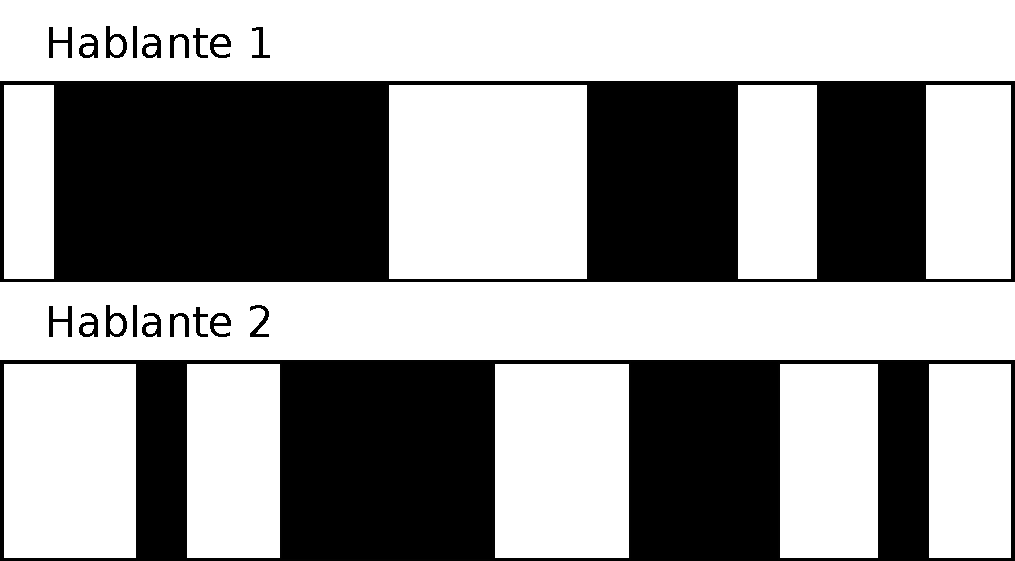
\includegraphics[scale=0.40]{images/conversation_turns.pdf}
  \end{figure}

  \begin{itemize}
    \item ¿Cómo comparamos los diferentes turnos de una conversación?
    \item Comparar uno a uno es un enfoque simplista y no representativo de la realidad
  \end{itemize}
\end{frame}

\begin{frame}
  \frametitle{Método TAMA}
\end{frame}


